% Preamble
\documentclass[11pt]{article}

% Packages
\usepackage{amsmath}
\usepackage[a4paper, margin=0.5in]{geometry}
\usepackage{graphicx}
\usepackage[utf8]{inputenc}
\usepackage[T1]{fontenc}
\usepackage[polish]{babel}
\usepackage{float}
\usepackage{hyperref}
\usepackage{cleveref}

\title{Projekt 1. UTA}
\author{Oskar Kiliańczyk 151863 \& Wojciech Kot 151876}
\date{}

% Document
\begin{document}

\maketitle
\newpage

\section{Opis informacji preferencyjnej}\label{sec:opis-informacji-preferencyjnej}

Z racji, że obaj wylosowaliśmy informację preferencyjną nr.\ 4, to firma przede wszystkim skupia się na preferowanej lokacji, gdzie:
\begin{itemize}
\item Lokalizacja R2 jest preferowana nad R1 oraz R1 nad R3.
\item Jako drugie, dodatkowe kryterium przyjęliśmy sposób finansowania, uznając metodę F1 (kWh-fee method) jako preferowaną ponad zarówno F2 (prorata method) oraz F3 (waste-fee method).
\end{itemize}

Pary referencyjne dobrane do naszego problemu to pary:
\begin{itemize}
\item przydzielone nam odgórnie:
\begin{itemize}
\item 11 i 14, gdzie 14 jest preferowane ponad 11 (R2 > R1)
\item 2 i 25, gdzie 2 jest preferowane ponad 25 (R1 > R3)
\end{itemize}
\item oraz wybrane przez nas:
\begin{itemize}
\item 11 i 17, gdzie 11 jest preferowane nad 17 (R2 > R3)
\end{itemize}
\item oraz dwie dla drugiego w ważności kryterium:
\begin{itemize}
\item 4 i 5, gdzie 4 jest preferowane nad 5 (R2=R2, F1 > F2)
\item 4 i 6,  gdzie 4 jest preferowane nad 6 (R2=R2, F1 > F3)
\end{itemize}
\end{itemize}

Na wartości wag dodaliśmy dodatkowe ograniczenia w postaci:
\begin{itemize}
\item wymuszenia monotoniczności (wszystkie kryteria są typu koszt).
\item normalizacji wag (aby użyteczność idealnego wariantu wynosiła 1, a antyidealnego 0).
\item dla każdego kryterium waga dla idealnego wariantu nie może być większa niż 0.5 (zapewniamy brak dominującego kryterium)
ani mniejsza niż 0.1 (zapewniamy że każde kryterium jest w jakimś stopniu ważne)
\end{itemize}


\section{Wynik uzyskany z solvera}\label{sec:wynik-uzyskany-z-solvera}
\subsection{UTA}
\begin{figure}[H]
	\centering
	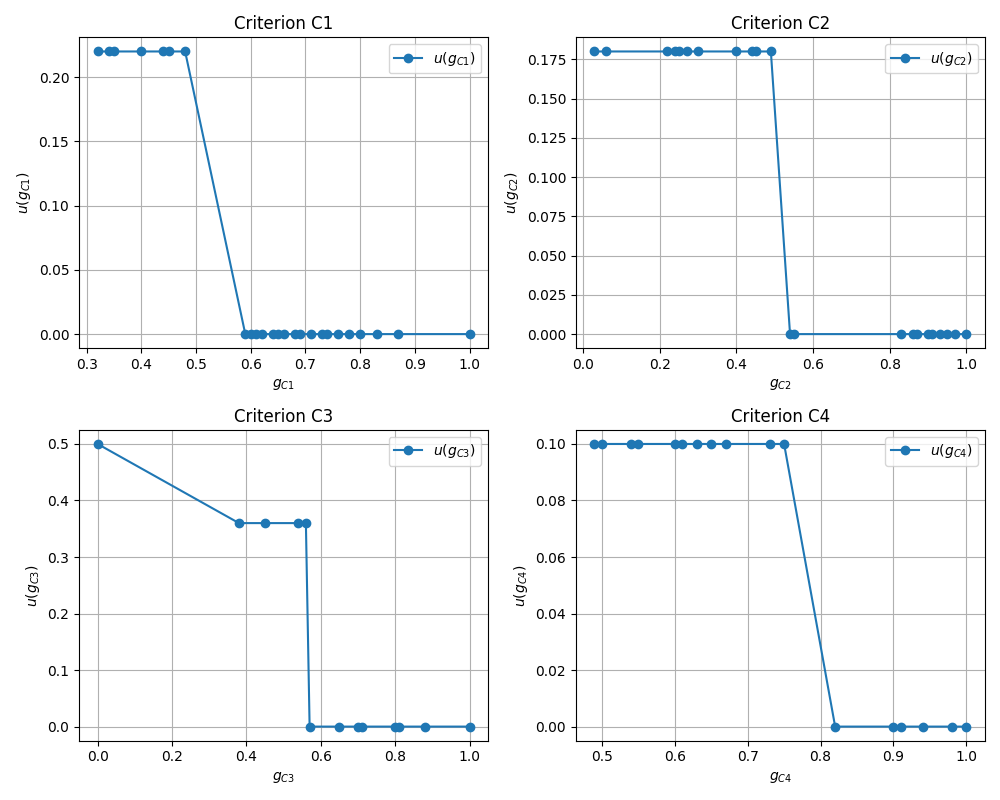
\includegraphics[scale=0.6]{uta.png}
\end{figure}

Tabela ~\ref{tab:utility_values} pokazuje uszeregowany ranking oraz wyniki wariantów dla poszczególnych kryteriów częściowych użyteczności. Ostatnia kolumna zawiera użyteczność całkowitą.
\begin{table}[H]
    \centering
    \begin{tabular}{|c|c|c|c|c|c|}
        \hline
        Alternatywa & C1  & C2  & C3  & C4  & $\Sigma$ \\
        \hline
        4  & 0.22 & 0.00 & 0.50 & 0.10 & 0.82 \\
        10 & 0.22 & 0.00 & 0.50 & 0.10 & 0.82 \\
        7  & 0.22 & 0.00 & 0.50 & 0.00 & 0.72 \\
        13 & 0.22 & 0.00 & 0.50 & 0.00 & 0.72 \\
        16 & 0.22 & 0.00 & 0.50 & 0.00 & 0.72 \\
        19 & 0.22 & 0.00 & 0.50 & 0.00 & 0.72 \\
        22 & 0.22 & 0.00 & 0.50 & 0.00 & 0.72 \\
        5  & 0.00 & 0.18 & 0.36 & 0.10 & 0.64 \\
        8  & 0.00 & 0.18 & 0.36 & 0.10 & 0.64 \\
        14 & 0.00 & 0.18 & 0.36 & 0.10 & 0.64 \\
        1  & 0.00 & 0.00 & 0.50 & 0.10 & 0.60 \\
        2  & 0.00 & 0.00 & 0.36 & 0.10 & 0.46 \\
        11 & 0.00 & 0.00 & 0.36 & 0.10 & 0.46 \\
        3  & 0.00 & 0.18 & 0.00 & 0.10 & 0.28 \\
        6  & 0.00 & 0.18 & 0.00 & 0.10 & 0.28 \\
        9  & 0.00 & 0.18 & 0.00 & 0.10 & 0.28 \\
        12 & 0.00 & 0.18 & 0.00 & 0.10 & 0.28 \\
        15 & 0.00 & 0.18 & 0.00 & 0.10 & 0.28 \\
        17 & 0.00 & 0.18 & 0.00 & 0.10 & 0.28 \\
        18 & 0.00 & 0.18 & 0.00 & 0.10 & 0.28 \\
        20 & 0.00 & 0.18 & 0.00 & 0.10 & 0.28 \\
        21 & 0.00 & 0.18 & 0.00 & 0.10 & 0.28 \\
        23 & 0.00 & 0.18 & 0.00 & 0.10 & 0.28 \\
        24 & 0.00 & 0.18 & 0.00 & 0.10 & 0.28 \\
        26 & 0.00 & 0.18 & 0.00 & 0.10 & 0.28 \\
        27 & 0.00 & 0.18 & 0.00 & 0.10 & 0.28 \\
        25 & 0.22 & 0.00 & 0.00 & 0.00 & 0.22 \\
        \hline
    \end{tabular}
    \caption{Użyteczności wszystkich wariantów oraz odpowiadające im częściowe użyteczności na podanych kryteriach}
    \label{tab:utility_values}
\end{table}

Celem optymalizacji była maksymalizacja najmniejszego dystansu między alternatywami silnie preferowanymi. Uzyskana wartość funkcji celu $\epsilon = 0.18$.

\section{Wyniki}\label{sec:wyniki}
Jeżeli chodzi o nasze pary referencyjne sytuacja wygląda następująco:
\begin{itemize}
\item Alternatywa 14 $\geq$ Alternatywa 11: $0.64 \geq 0.46$
\item Alternatywa 2 $\geq$ Alternatyw 25: $0.46 \geq 0.22$
\item Alternatywa 11 $\geq$ Alternatyw 17: $0.46 \geq 0.28$
\item Alternatywa 4 $\geq$ Alternatyw 5: $0.82 \geq 0.64$
\item Alternatywa 4 $\geq$ Alternatyw 6: $0.82 \geq 0.28$
\end{itemize}

Otrzymany ranking został sprawdzony dla innych niereferencyjnych par, w celu otrzymania spójnej informacji preferencyjnej.
\begin{itemize}
\item Alternatywa 7 $\geq$ Alternatywa 8: $0.72 \geq 0.64$ --- co potwierdza $F1 > F2$, przy równości R3.
\item Alternatywa 13 $\geq$ Alternatywa 25: $0.72 \geq 0.22$ --- co potwierdza $R2 > R3$, przy równości F1.
\end{itemize}
Były jednak także odstępstwa, przykładowo:
\begin{itemize}
\item Alternatywa 13 $\not\geq$ Alternatywa 10: $0.72 \not\geq $ 0.82 --- przy równości F1, obserwujemy $R1 > R2$, co jest sprzeczne z informacją preferencyjną.
\end{itemize}

Najlepszą ocenę użyteczności globalnej uzyskały warianty alternatyw o numerach 4 (R2, F1) i 10 (R1, F1). Ze względu na ocenę na poszczególnych kryteriach dostały one najwyższą wartość dla kryteriów C1, C3 oraz C4.

Najgorszą ocenę użyteczności globalnej uzyskał wariant alternatywy o numerze 25 (R3, F1), uzyskując jedynie pozytywny wynik dla kryterium C1. Warto zauważyć, że drugi wynik od końca z oceną użyteczności na poziomie 0.28 klasyfikuje wiele alternatyw, które otrzymały odpowiednio wynik dla kryteriów C2 oraz C4.

Widać zależności:
\begin{itemize}
\item Ze względu na wagę kryterium C3, alternatywy najwyżej w klasyfikacji otrzymały na nim najwięcej oceny użyteczności cząstkowej.
\item Kryterium C4 było mało znaczące i prawie każda alternatywa (z wyłączeniem 6 z nich) otrzymała maksymalną możliwą wartość na tym kryterium.
\item Najwyżej wycenione alternatywy cechują się maksymalną użytecznością cząstkową na kryterium C1, C3 i C4.
\end{itemize}

Warto zauważyć, że otrzymanie najwyższej możliwej użyteczności częściowej dla kryterium C3 w wysokości $0.5$ już dawał możliwość uzyskania 11 pozycji z 27 w klasyfikacji ogólnej. Pomimo, że użyteczność na tym kryterium spada jest możliwość uzyskania wysokich, w stosunku do całej użyteczności globalnej, wyników. 

\subsection{UTA-GMS i diagram Hasse'ego}
W celu uzyskania relacji koniecznych dodano nowe ograniczenie. Prócz typowych ograniczeń związanych z definicją problemu dodajemy nową zmienną $\sigma$, która będzie minimalizowana. Dla każdej pary wariantów minimalizujemy różnicę pomiędzy ich użytecznościami globalnymi i rozwiązujemy problem. Jeżeli jego wartość jest większa lub równa 0, oznacza to że relacja $A_i$ jest koniecznie preferowane nad $A_j$. Po przejściu przez każdą możliwą parę wariantów uzyskujemy pełną listę relacji koniecznie preferowanych. Z tej listy generujemy diagram Hasse'ego.
\begin{figure}[H]
	\centering
	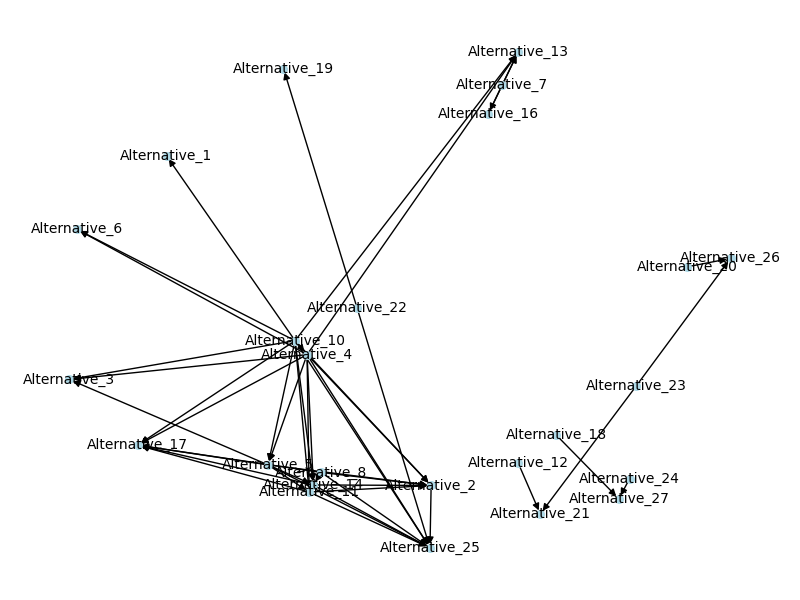
\includegraphics[scale=0.6]{hasse.png}
\end{figure}

W naszym przypadku liczba takich relacji koniecznie preferowanych jest równa aż 50, stąd trudności z dobrą wizualizacją diagramu. Jesteśmy w stanie zaobserwować podobne efekty, które widzieliśmy w użytecznościach globalnych standardowego problemu UTA. Można zaobserwować ,,wyższość'' alternatyw 10 i 4. Dodatkowo alternatywy numer 8 i 5 przewyższają wiele innych. Może być to spowodowane maksymalną użytecznością częściową dla kryteriów C2, C3 i C4. Można obserwować liczne alternatywy będące przewyższane, których użyteczności globalne są niskie i znajdują się na dole tabeli ~\ref{tab:utility_values}

\subsection{Reprezentatywna funkcja użyteczności}
\begin{figure}[H]
	\centering
	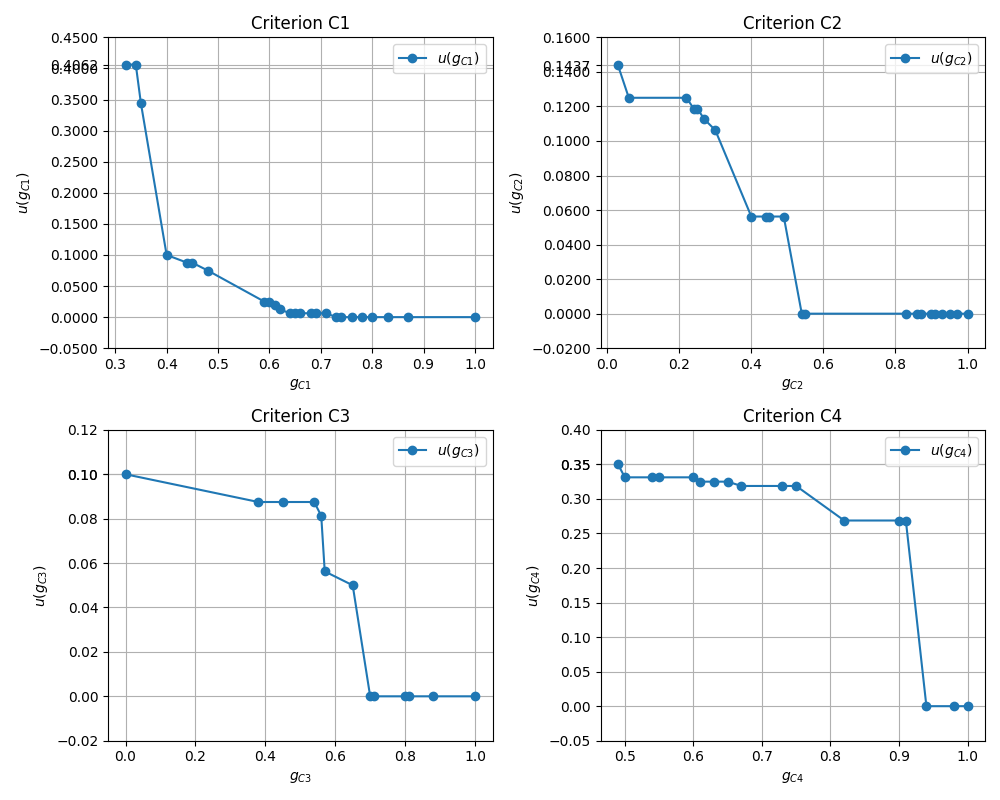
\includegraphics[scale=0.6]{representative_function.png}
\end{figure}
Zasadniczą różnicą, którą widać na pierwszy rzut oka względem wersji UTA, to zmiana drastyczna wag. Kryterium C1 jest teraz bardziej znaczące, lecz tylko dla wariantów najlepszych, dla reszty z nich jest znacznie mniej nagradzająca. Krterium C3 nie jest już na maksymalnym poziomie wartości funkcji użyteczności 0.5. Zamiast tego straciło znacznie na swojej wartości, zachowując jednak swój kształt. Kryterium 4 jest teraz bardziej znaczące i nagradza znacznie praktycznie wszystkie alternatywy.

\begin{table}[H]
    \centering
    \begin{tabular}{|c|c|c|c|c|c|}
        \hline
        Alternatywa & C1  & C2  & C3  & C4  & $\Sigma$ \\
        \hline
        10 & 0.0875 & 0.00 & 0.10 & 0.31875 & 0.50625 \\
        22 & 0.40625 & -0.00 & 0.10 & 0.00 & 0.50625 \\
        4  & 0.075 & -0.00 & 0.10 & 0.31875 & 0.49375 \\
        5  & 0.0125 & 0.05625 & 0.08125 & 0.33125 & 0.48125 \\
        8  & 0.00625 & 0.05625 & 0.0875 & 0.33125 & 0.48125 \\
        7  & 0.10 & 0.00 & 0.10 & 0.26875 & 0.46875 \\
        12 & 0.00 & 0.11875 & 0.00 & 0.35 & 0.46875 \\
        14 & 0.00625 & 0.05625 & 0.08125 & 0.325 & 0.46875 \\
        15 & 0.00 & 0.14375 & 0.00 & 0.325 & 0.46875 \\
        23 & 0.025 & 0.11875 & 0.00 & 0.325 & 0.46875 \\
        24 & 0.00 & 0.14375 & 0.00 & 0.325 & 0.46875 \\
        11 & 0.01875 & 0.00 & 0.0875 & 0.35 & 0.45625 \\
        16 & 0.0875 & 0.00 & 0.10 & 0.26875 & 0.45625 \\
        18 & 0.00 & 0.125 & 0.00 & 0.33125 & 0.45625 \\
        20 & 0.00625 & 0.125 & 0.00 & 0.325 & 0.45625 \\
        1  & 0.025 & 0.00 & 0.10 & 0.31875 & 0.44375 \\
        2  & 0.00625 & 0.00 & 0.0875 & 0.35 & 0.44375 \\
        3  & 0.00 & 0.05625 & 0.05625 & 0.33125 & 0.44375 \\
        6  & 0.00 & 0.1125 & 0.00 & 0.33125 & 0.44375 \\
        9  & 0.00625 & 0.10625 & 0.00 & 0.33125 & 0.44375 \\
        13 & 0.075 & 0.00 & 0.10 & 0.26875 & 0.44375 \\
        17 & 0.00625 & 0.05625 & 0.05 & 0.33125 & 0.44375 \\
        19 & 0.34375 & -0.00 & 0.10 & 0.00 & 0.44375 \\
        21 & 0.00 & 0.11875 & 0.00 & 0.325 & 0.44375 \\
        26 & 0.00625 & 0.11875 & 0.00 & 0.31875 & 0.44375 \\
        27 & 0.00 & 0.125 & 0.00 & 0.31875 & 0.44375 \\
        25 & 0.40625 & 0.00 & 0.00 & 0.00 & 0.40625 \\
        \hline
    \end{tabular}
    \caption{Funkcja reprezentatywna użyteczności}
    \label{tab:representative_utility}
\end{table}

Obserwując wyniki z tabeli ~\ref{tab:representative_utility} można zaobserwować, że reprezentatywna funkcja użyteczności sprowadza globalną użyteczność alternatyw, to jest różnice między poszczególnymi parami, do minimum. Rozstrzał wartości jest nieznaczny. Można zaobserwować, że alternatywy z najwyższą użytecznością globalną dla problemu z zadania 3 mają również tutaj zachowaną wysoką użyteczność globalną. To samo tyczy się alternatyw o najniższej użyteczności globalnej. Alternatywy znajdujące się w środku rankingu mogły zmienić swoją pozycję, lecz w ograniczonym stopniu, a różnice pomiędzy poszczególnymi alternatywami (ich użytecznościami globalnymi) jest niewielki.

Jeżeli chodzi o nasze pary referencyjne sytuacja wygląda następująco:
\begin{itemize}
\item Alternatywa 14 $\geq$ Alternatywa 11: $0.46875 \geq 0.45625$
\item Alternatywa 2 $\geq$ Alternatywa 25: $0.44375 \geq 0.40625$
\item Alternatywa 11 $\geq$ Alternatywa 17: $0.45625 \geq 0.44375$
\item Alternatywa 4 $\geq$ Alternatywa 5: $0.49375 \geq 0.48125$
\item Alternatywa 4 $\geq$ Alternatywa 6: $0.49375 \geq 0.44375$
\end{itemize}

\section{Link do repozytorium}\label{sec:link-do-repo}
Kod źródłowy w repozytorium GitHub dostępny pod linkiem: \\
\href{https://github.com/KotZPolibudy/PUT_ISWD/tree/main/projekt1}{Repozytorium ISWD - projekt 1}.


\end{document}
